\documentclass[12pt,a4paper]{article}

\usepackage[utf8]{inputenc}
\usepackage[T1]{fontenc}
\usepackage[english]{babel}
\usepackage{amsmath,amssymb}
\usepackage{bm}
\usepackage[margin=2.5cm]{geometry}
\usepackage{booktabs}
\usepackage{array}
\usepackage{xcolor}
\usepackage{hyperref}
\usepackage{float}
\usepackage{enumitem}
\usepackage{listings}
\usepackage{caption}
\usepackage{subcaption}
\usepackage[numbers,sort&compress]{natbib}
\usepackage{fancyhdr}
\usepackage{parskip}
\usepackage{rotating}
\usepackage{graphicx}
\graphicspath{{../notebooks/figures/}}

\hypersetup{colorlinks=true,linkcolor=blue!70!black,
  citecolor=green!50!black,urlcolor=blue!70!black}

\definecolor{codebg}{RGB}{248,248,248}
\lstdefinestyle{pythonstyle}{
  backgroundcolor=\color{codebg},basicstyle=\ttfamily\small,
  keywordstyle=\bfseries,frame=single,breaklines=true,
  language=Python,showstringspaces=false,
  numbers=left,numberstyle=\tiny\color{gray},xleftmargin=2em}
\lstset{style=pythonstyle}

\pagestyle{fancy}\fancyhf{}
\rhead{\small Bayesian Neural Networks}
\lhead{\small Implementations using Python Libraries}
\cfoot{\thepage}
\setlength{\headheight}{14.5pt}

\newcommand{\btheta}{\bm{\theta}}
\newcommand{\cD}{\mathcal{D}}
\newcommand{\cN}{\mathcal{N}}
\newcommand{\KL}{\mathrm{KL}}
\newcommand{\ELBO}{\mathcal{L}_{\text{ELBO}}}
\newcommand{\MAP}{\text{MAP}}
\newcolumntype{C}[1]{>{\centering\arraybackslash}p{#1}}
\newcolumntype{L}[1]{>{\raggedright\arraybackslash}p{#1}}
\newcommand{\todo}[1]{\noindent\colorbox{yellow!40}{\parbox{\dimexpr\linewidth-2\fboxsep}{\textbf{[TODO]} #1}}}

\begin{document}

\begin{titlepage}
  \centering\vspace*{2cm}
  {\LARGE\bfseries Bayesian Neural Networks:\\[4pt]
   \texttt{Implementations using Python Libraries}\par}
  \vspace{0.8cm}
  \vspace{2cm}
  \rule{0.7\linewidth}{0.4pt}\\[0.4cm]
  {\normalsize\today}
\end{titlepage}

\tableofcontents
\newpage

%% ═══════════════════════════════════════════════════════════════════════════
\section{Introduction}
\label{sec:intro}

Standard deep neural networks are notoriously miscalibrated: high-confidence
predictions are not guaranteed to be correct, and models frequently fail
silently under distribution shift~\citep{goan2020bayesian,murphy2023pml}.
Bayesian Deep Learning (BDL) addresses this by replacing a deterministic weight
estimate with a posterior distribution $p(\btheta \mid \cD)$, propagating weight
uncertainty into calibrated predictive distributions.

This report compares two PyTorch libraries implementing complementary BDL
paradigms:
\begin{itemize}[leftmargin=*]
  \item \textbf{\texttt{bayesian-torch}}~\citep{intel2021bayesiantorch}, a
        ``Bayesian-by-design'' library from Intel Labs implementing mean-field
        Variational Inference via Flipout~\citep{wen2018flipout} and
        Bayes-by-Backprop (BBB)~\citep{blundell2015weight}.
  \item \textbf{\texttt{laplace-torch}}~\citep{daxberger2021laplace,aleximmer2024laplace},
        a post-hoc library applying the Laplace Approximation (LA) to any
        pre-trained model without modifying its training loop.
\end{itemize}

Experiments span three settings: (i)~a synthetic binary classification
benchmark (Two Moons, \S\ref{sec:twomoons}), (ii)~\todo{a toy regression
experiment (\S\ref{sec:regression})}, and (iii)~\todo{a replication of the
Laplace Redux PovertyMap experiment (\S\ref{sec:povertymap})}.
Full metric tables and figure galleries for completed experiments are in the
Appendix.

%% ───────────────────────────────────────────────────────────────────────────
\section{Theoretical Background}
\label{sec:theory}

\subsection{Bayesian Deep Learning}

Given $\cD = \{(\bm{x}_n, y_n)\}_{n=1}^{N}$ and network $f_{\btheta}$, the
posterior is $p(\btheta \mid \cD) = p(\cD|\btheta)\,p(\btheta)/p(\cD)$. The
evidence is intractable for modern DNNs. With a Gaussian prior
$p(\btheta)=\cN(\bm{0},\tau^{-1}\mathbf{I})$, the MAP estimate
$\btheta_{\MAP} = \arg\max_{\btheta}[\log p(\cD|\btheta)+\log p(\btheta)]$
corresponds to $L_2$-regularised training with weight decay
$\lambda=\tau$~\citep{murphy2023pml}.

\subsection{Stochastic Variational Inference}

VI approximates the posterior with a tractable family $q_{\bm\phi}(\btheta)$
by maximising the Evidence Lower Bound~\citep{blundell2015weight,goan2020bayesian}:
\begin{equation}
  \ELBO(\bm\phi)
    = \mathbb{E}_{q}\!\bigl[\log p(\cD|\btheta)\bigr]
    - \KL\bigl(q_{\bm\phi}\,\|\,p(\btheta)\bigr).
  \label{eq:elbo}
\end{equation}
A mean-field Gaussian $q_{\bm\phi}(w_i) = \cN(\mu_i,\sigma_i^2)$ with
$\sigma_i = \log(1+\exp(\rho_i))>0$ keeps the KL in~\eqref{eq:elbo} in
closed form, but doubles the parameter count ($\mu_i$ and $\rho_i$ per
weight).

\subsubsection{Bayes by Backprop (BBB)}

\citet{blundell2015weight} reparameterise each weight as
\begin{equation}
  w_i = \mu_i + \sigma_i\,\varepsilon_i, \qquad \varepsilon_i\sim\cN(0,1),
\end{equation}
enabling low-variance gradient estimates of~\eqref{eq:elbo} via
backpropagation. A single noise draw is shared across all examples in a
mini-batch, which inflates gradient variance at large batch sizes.

\subsubsection{Flipout}

\citet{wen2018flipout} reduce this variance by applying independent sign-flip
matrices $\mathbf{r}_n,\mathbf{s}_n\in\{-1,+1\}^*$ to the shared
perturbation $\Delta\hat{\mathbf{W}}$ for each example $n$:
\begin{equation}
  \hat{\mathbf{W}}_n
    = \mathbf{W}_{\MAP} + \mathbf{s}_n \odot \Delta\hat{\mathbf{W}}
      \odot \mathbf{r}_n^{\!\top}.
\end{equation}
The key result from~\citet{wen2018flipout} (Theorem~2) is that Flipout's
gradient variance scales as $\mathcal{O}(1/N_{\mathcal{B}})$ with batch size
$N_{\mathcal{B}}$, identical to fully independent perturbations, at only
$\mathcal{O}(1)$ extra cost per layer. Plain BBB variance, by contrast,
levels off to a constant once the shared-perturbation term dominates.

\subsubsection{MOPED Initialisation}

Training mean-field BNNs from random initialisations is fragile: the ELBO
landscape has flat regions and the KL term can dominate early training.
\texttt{bayesian-torch}~\citep{intel2021bayesiantorch} addresses this via
\textbf{MOPED}: the posterior means $\{\mu_i\}$ are warm-started from a
pre-trained MAP checkpoint and the prior scale is set proportionally:
\begin{equation}
  \mu_i^{(0)} = \theta_{\MAP}^{(i)}, \qquad
  \sigma_i^{\text{prior}} = \delta\,|\theta_{\MAP}^{(i)}|, \quad \delta=0.5.
\end{equation}
This provides a principled empirical-Bayes starting point, drastically
reducing the required number of training epochs (100-epoch cap vs.\ 300 for
scratch training) and, as shown experimentally, preventing posterior collapse
under the AvUC objective.

\subsubsection{AvUC Loss}
\label{sec:theory:avuc}

Standard ELBO training minimises NLL but does not explicitly calibrate the
relationship between confidence and accuracy. The
\textbf{Accuracy-vs-Uncertainty Calibration (AvUC)} loss, implemented in
\texttt{bayesian-torch}~\citep{intel2021bayesiantorch}, adds a direct
penalty for miscalibrated confidence.

\paragraph{Predictive quantities.}
Given $M$ MC forward passes, compute the mean predictive probability:
\begin{equation}
  \bar{\mathbf{f}}_n = \frac{1}{M}\sum_{m=1}^{M} f_{\btheta_m}(\bm{x}_n),
  \qquad \hat{p}_n = \mathrm{softmax}(\bar{\mathbf{f}}_n),
\end{equation}
and the predictive entropy of each sample ($M=5$ in all experiments):
\begin{equation}
  H_n = -\sum_{c=1}^{C} \hat{p}_{nc}\,\log\hat{p}_{nc}.
\end{equation}

\paragraph{Calibration quadrants.}
A batch-level uncertainty threshold is computed as the mean entropy:
\begin{equation}
  \hat{\kappa} = \frac{1}{|\mathcal{B}|}\sum_{n\in\mathcal{B}} H_n.
\end{equation}
Each prediction is then assigned binary accuracy and uncertainty indicators:
\begin{equation}
  a_n = \mathbf{1}\bigl[\arg\max_c\hat{p}_{nc} = y_n\bigr], \qquad
  u_n = \mathbf{1}[H_n \geq \hat{\kappa}],
\end{equation}
yielding four calibration quadrants:
\begin{center}
  \renewcommand{\arraystretch}{1.3}
  \begin{tabular}{rcc}
    \toprule
                           & Certain ($u_n=0$)      & Uncertain ($u_n=1$)     \\
    \midrule
    Accurate ($a_n=1$)     & AC \checkmark          & AU \texttimes           \\
    Inaccurate ($a_n=0$)   & IC \texttimes          & IU \checkmark           \\
    \bottomrule
  \end{tabular}
\end{center}
AC (accurate, certain) and IU (inaccurate, uncertain) are desirable;
AU (accurate but over-uncertain) and IC (inaccurate but overconfident) are
penalised.

\paragraph{AvUC objective.}
The AvUC loss aggregates the fractions of samples in the two
``bad'' quadrants~\citep{intel2021bayesiantorch}:
\begin{equation}
  \mathcal{L}_{\mathrm{AvUC}}
    = \underbrace{\frac{n_{AU}}{n_{AU}+n_{AC}}}_{\text{over-uncertain among correct}}
    + \underbrace{\frac{n_{IC}}{n_{IC}+n_{IU}}}_{\text{overconfident among wrong}},
  \label{eq:avuc}
\end{equation}
where $n_X$ counts samples in quadrant $X$ within the current mini-batch.
Each term lies in $[0,1]$; both are zero when calibration is perfect.

\paragraph{Full training objective.}
The combined loss is:
\begin{equation}
  \mathcal{L}
    = \underbrace{-\frac{1}{|\mathcal{B}|}\sum_{n\in\mathcal{B}}
        \log\hat{p}_{n,y_n}}_{\mathcal{L}_{\mathrm{CE}}}
    + \underbrace{\frac{\KL(q_{\bm\phi}\|p)}{N}}_{\text{ELBO regulariser}}
    + \underbrace{\mathcal{L}_{\mathrm{AvUC}}}_{\text{calibration}},
  \label{eq:avuc_total}
\end{equation}
where $N$ is the total training set size (scaling the KL to match
per-example CE).

\paragraph{Computational cost.}
Because $\hat{p}_n$ in~\eqref{eq:avuc} requires the mean over $M=5$ MC
samples, AvUC multiplies the per-step compute by a factor of $\approx M$
relative to the single-sample ELBO, explaining the $\approx 4\times$ increase
in wall-clock training time observed in all experiments.

\subsection{Epistemic and Aleatoric Uncertainty Decomposition}
\label{sec:theory:unc_decomp}

For MC-based BNNs, the total predictive uncertainty can be decomposed into
two orthogonal components~\citep{goan2020bayesian}:
\begin{align}
  \text{Total}   &= H\!\left[\frac{1}{S}\sum_{s=1}^{S} p(y|f_{\btheta_s}(\bm{x}))\right], \\
  \text{Aleatoric}&= \frac{1}{S}\sum_{s=1}^{S} H\!\left[p(y|f_{\btheta_s}(\bm{x}))\right], \\
  \text{Epistemic}&= \text{Total} - \text{Aleatoric}
    = I\!\left(y;\btheta\,|\,\bm{x},\cD\right),
  \label{eq:mi}
\end{align}
where $I$ is the mutual information between labels and weights given the
input. Equation~\eqref{eq:mi} is precisely what is plotted in the
``OOD epistemic uncertainty'' maps: regions with large $I$ signal that
the model's own weight samples disagree on the prediction: the signature
of a genuinely unknown input.

\subsection{Laplace Approximation}
\label{sec:theory:la}

The LA~\citep{daxberger2021laplace} builds a Gaussian posterior around
$\btheta_{\MAP}$ via second-order Taylor expansion:
\begin{equation}
  p(\btheta|\cD) \approx \cN\!\bigl(\btheta;\,\btheta_{\MAP},\,\mathbf{H}^{-1}\bigr),
  \qquad
  \mathbf{H} = -\nabla^2\log p(\btheta_{\MAP}|\cD) \succ 0.
\end{equation}
No modification to the training loop is required; the MAP network is frozen
and the curvature is estimated post-hoc via a single pass through the
training data.

\paragraph{GGN and Hessian structure.}
\texttt{laplace-torch}~\citep{aleximmer2024laplace} approximates $\mathbf{H}$
with the positive semi-definite Generalised Gauss--Newton (GGN) matrix and
offers four factorisation schemes (Table~\ref{tab:hessian}).

\begin{table}[H]
  \centering
  \caption{Hessian factorisation options in \texttt{laplace-torch}.}
  \label{tab:hessian}
  \small
  \begin{tabular}{lll}
    \toprule
    \textbf{Structure} & \textbf{Memory} & \textbf{Notes} \\
    \midrule
    Full     & $\mathcal{O}(P^2)$                       & Exact GGN; infeasible for large nets \\
    KFAC     & $\mathcal{O}(\sum_l N_l^2+N_{l-1}^2)$   & Per-layer Kronecker product; recommended \\
    Diagonal & $\mathcal{O}(P)$                          & Fastest; ignores off-diagonal correlations \\
    Low-Rank & $\mathcal{O}(Pk)$                         & Top-$k$ eigendecomposition of GGN \\
    \bottomrule
  \end{tabular}
\end{table}

\paragraph{Marginal likelihood tuning.}
The prior precision $\tau$ is selected by maximising the log-evidence:
\begin{equation}
  \log p(\cD)
    \approx \log p(\cD|\btheta_{\MAP})
    + \log p(\btheta_{\MAP})
    + \tfrac{P}{2}\log 2\pi
    - \tfrac{1}{2}\log\det\mathbf{H},
  \label{eq:marglik}
\end{equation}
which is differentiable with respect to $\tau$ and requires no validation
data~\citep{daxberger2021laplace}. Grid search over
a discrete set of values on validation NLL is simpler but requires a
held-out split.

\paragraph{Predictive approximation.}
All experiments use the probit approximation to the softmax-Gaussian
integral~\citep{daxberger2021laplace}, which is closed-form and exact for
the Last-Layer LA.

%% ───────────────────────────────────────────────────────────────────────────
\section{Evaluation Metrics}
\label{sec:metrics}

\paragraph{Accuracy / NLL.}
$\mathrm{NLL}=-\frac{1}{N}\sum_n\log\hat{p}(y_n|\bm{x}_n)$; lower is better.

\paragraph{Brier Score.}
$\mathrm{BS}=\frac{1}{N}\sum_n\sum_c(\hat{p}_{nc}-\mathbf{1}[y_n=c])^2$;
bounded and less sensitive to extreme probabilities than NLL.

\paragraph{ECE.}
Predictions binned into $B=15$ equal-width confidence bins; weighted mean
of $|\overline{\mathrm{acc}}_b-\overline{\mathrm{conf}}_b|$.
Perfect calibration gives ECE$=0$.

\paragraph{Reliability diagram.}
Visual companion to ECE: plots binned accuracy against mean confidence.
A perfectly calibrated model traces the diagonal.

\paragraph{Mean Confidence / Mean Entropy / $1-\text{Confidence}$.}
Mean max-class probability, mean Shannon entropy $H$, and
$1-\max_c\hat{p}_c\in[0,0.5]$ (direct uncertainty proxy).

\paragraph{Uncertainty calibration (U-MAE, U-MSE, U-Corr, Max Gap).}
Compares expected uncertainty ($1-\text{conf}$) against empirical error rate
per bin. Pearson correlation and max bin gap assess worst-case alignment.

\paragraph{Epistemic uncertainty (OOD maps).}
Mutual information $I(y;\btheta|\bm{x},\cD)$ estimated via
equation~\eqref{eq:mi} with $S=50$ MC samples.

\paragraph{Timing.}
Fit time (VI training or Hessian computation), tune time (prior precision
optimisation), and inference time per full test batch.

%% ───────────────────────────────────────────────────────────────────────────
\section{Shared Infrastructure}
\label{sec:shared}

Both notebooks share a \texttt{shared} utility package.

\paragraph{TinyMLP.}
\texttt{Linear(2,64)$\to$Tanh$\to$Linear(64,64)$\to$Tanh$\to$Linear(64,2)};
4\,482 parameters, expanding to 8\,964 after \texttt{dnn\_to\_bnn}
($\mu_i$ and $\rho_i$ per weight).

\paragraph{MAP baseline.}
Adam, lr$=10^{-3}$, up to 300 epochs, early stopping on validation NLL.
Fit time: $33.6$\,s. The same checkpoint is reused by both notebooks.

%% ───────────────────────────────────────────────────────────────────────────
\section{Two Moons Classification}
\label{sec:twomoons}

\subsection{Dataset and OOD Probe Design}

2\,000 2-D points from two interleaved half-crescents
(\texttt{make\_moons}, noise$=0.3$, seed$=42$), split 60/20/20.
The non-linear decision boundary is the canonical stress-test for
uncertainty quantification.

To probe out-of-distribution (OOD) behaviour, 200 probe points are
sampled in four corner clusters at $\|x\|_\infty \approx 3$--$4$,
deliberately outside the training manifold (Figure~\ref{fig:ood_points}).

\begin{figure}[H]
  \centering
  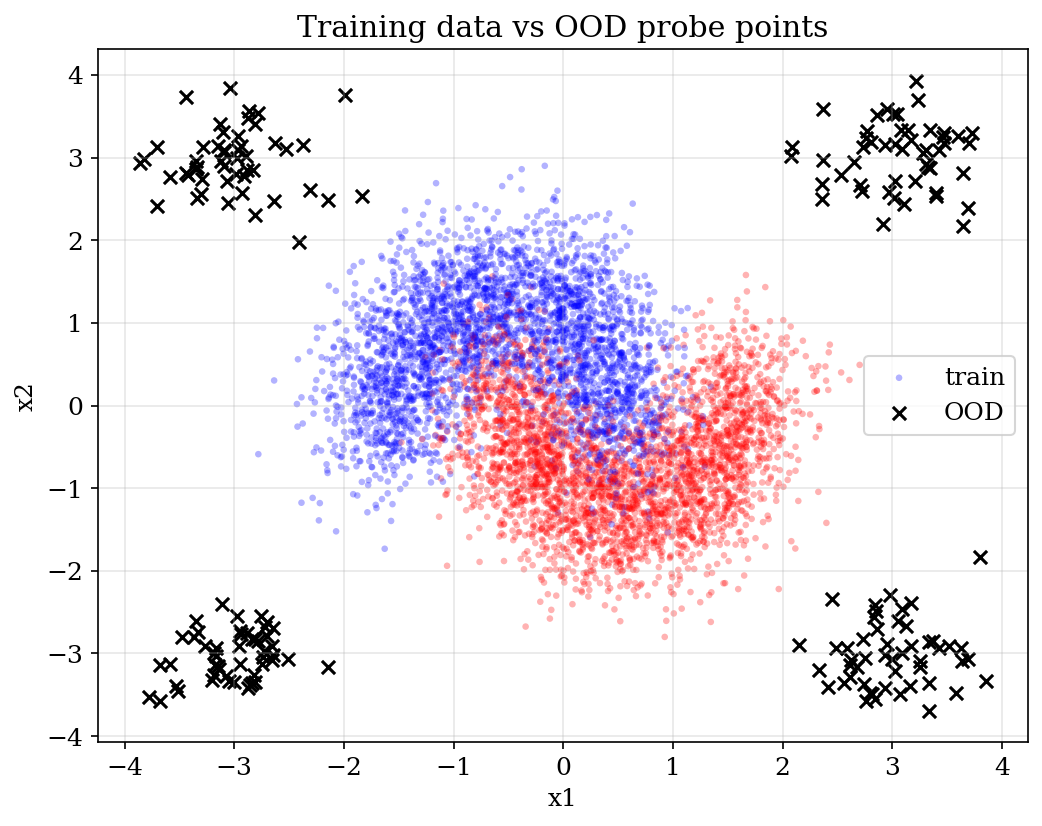
\includegraphics[width=0.60\linewidth]{ood_points.png}
  \caption{Training data (coloured dots) and OOD probe points ($\times$).
    OOD clusters are placed in the four corners of the input space, well
    outside the training support.}
  \label{fig:ood_points}
\end{figure}

%% ── 4.2 bayesian-torch ────────────────────────────────────────────────────
\subsection{\texttt{bayesian-torch}: Variational BNN}
\label{sec:bnn}

\paragraph{Setup.}
\texttt{dnn\_to\_bnn()} converts every \texttt{nn.Linear} to a variational
layer. Inference uses $S=50$ MC forward passes. Eight variants cross
Estimator$\in$\{Flipout, BBB\} $\times$ Init$\in$\{scratch, MOPED\}
$\times$ Loss$\in$\{ELBO, ELBO+AvUC\}.

\begin{lstlisting}[caption={BNN conversion and ELBO/AvUC training (BBB shown).}]
dnn_to_bnn(net, {"prior_mu": 0.0, "prior_sigma": 1.0,
    "posterior_mu_init": 0.0, "posterior_rho_init": -3.0,
    "type": "Reparameterization",          # or "Flipout"
    "moped_enable": True, "moped_delta": 0.5})

# ELBO step
loss = criterion(net(inputs), labels) + get_kl_loss(net) / N

# AvUC step (M=5 MC samples)
logits_mc = torch.stack([net(inputs) for _ in range(5)], dim=0)
mean_logits = logits_mc.mean(dim=0)
probs = torch.softmax(mean_logits, dim=1)
ent = -(probs * torch.log(probs + 1e-12)).sum(dim=1)
khat = ent.mean().item()          # batch-level threshold kappa
avu  = AvULoss()(mean_logits, labels, khat, type=0)
loss = CE(mean_logits, labels) + get_kl_loss(net) / N + avu
\end{lstlisting}

\paragraph{Results.}

Tables~\ref{tab:bnn_main} and~\ref{tab:bnn_ood} report all calibration and
OOD metrics for all eight variants. U-MSE values are scaled by $10^3$ for
readability. Bold marks the best value in each metric column.

\begin{sidewaystable}
  \centering
  \caption{All calibration metrics for \texttt{bayesian-torch} variants on
    Two Moons ($S=50$ MC samples). Bold = best per column.}
  \label{tab:bnn_main}
  \scriptsize\setlength{\tabcolsep}{2.5pt}
  \begin{tabular}{
    L{1.5cm} C{0.6cm} C{0.65cm}
    C{0.65cm} C{0.7cm} C{0.7cm} C{0.7cm}
    C{0.7cm} C{0.7cm} C{0.65cm}
    C{0.7cm} C{0.95cm} C{0.7cm}
    C{0.75cm} C{0.7cm} C{0.75cm}
    C{0.5cm} C{0.9cm} C{0.85cm}
  }
    \toprule
    \textbf{Type} & \textbf{Init} & \textbf{Loss}
      & \textbf{Acc} & \textbf{NLL} & \textbf{BS} & \textbf{ECE}
      & \textbf{Conf} & \textbf{Ent} & \textbf{$1{-}c$}
      & \textbf{U-MAE} & \textbf{U-MSE}${\times}10^3$ & \textbf{U-Corr}
      & \textbf{MaxGap} & \textbf{ClECE} & \textbf{MActErr}
      & \textbf{Ep} & \textbf{Fit\,(s)} & \textbf{Inf\,(s)} \\
    \midrule
    \multicolumn{19}{l}{\textit{Flipout estimator}} \\
    Flipout & scr & ELBO & 0.921 & 0.198 & 0.058 & 0.018 & 0.906 & 0.241 & 0.094 & 0.018 & 0.458 & 0.988 & 0.069 & 0.018 & 0.080 & 39 & 19.1 & 0.064 \\
    Flipout & scr & AvUC & 0.918 & 0.198 & 0.059 & 0.014 & 0.928 & 0.184 & 0.072 & 0.014 & 0.840 & 0.953 & 0.134 & 0.014 & 0.082 & 38 & 80.4 & 0.065 \\
    Flipout & MOP & ELBO & 0.918 & 0.199 & 0.059 & 0.019 & 0.911 & 0.222 & 0.089 & 0.019 & 0.882 & 0.935 & 0.113 & 0.019 & 0.083 & 39 & 20.0 & 0.063 \\
    Flipout & MOP & AvUC & 0.920 & 0.201 & 0.059 & \textbf{0.010} & 0.928 & 0.184 & 0.072 & \textbf{0.010} & \textbf{0.294} & \textbf{0.990} & 0.078 & \textbf{0.010} & 0.081 & 40 & 90.1 & 0.064 \\
    \multicolumn{19}{l}{\textit{Reparameterisation (BBB) estimator}} \\
    BBB & scr & ELBO & \textbf{0.923} & 0.197 & 0.058 & 0.019 & 0.911 & 0.229 & 0.088 & 0.019 & 0.582 & 0.983 & \textbf{0.051} & 0.019 & 0.078 & 50 & 23.2 & 0.051 \\
    BBB & scr & AvUC & 0.866 & 0.311 & 0.095 & 0.028 & 0.847 & 0.362 & 0.153 & 0.028 & 0.918 & 0.965 & 0.102 & 0.028 & 0.134 & 32 & 73.3 & 0.050 \\
    BBB & MOP & ELBO & 0.920 & 0.195 & 0.058 & 0.015 & 0.913 & 0.217 & 0.087 & 0.015 & 0.556 & 0.967 & 0.130 & 0.015 & 0.081 & 36 & \textbf{15.9} & 0.055 \\
    \textbf{BBB} & \textbf{MOP} & \textbf{AvUC} & \textbf{0.923} & \textbf{0.192} & \textbf{0.057} & 0.014 & \textbf{0.933} & \textbf{0.173} & \textbf{0.067} & 0.014 & 0.900 & 0.941 & 0.123 & 0.014 & \textbf{0.078} & 33 & 68.7 & 0.051 \\
    \bottomrule
  \end{tabular}
  \begin{flushleft}\footnotesize
    scr = random init; MOP = MOPED warm-start.
    Ep = epochs run (early stopping). U-MSE scaled by $10^3$.
    MaxGap = max binned uncertainty gap. ClECE = classwise ECE.
    MActErr = mean actual error rate.
  \end{flushleft}
\end{sidewaystable}

\begin{table}[H]
  \centering
  \caption{OOD epistemic uncertainty decomposition for all
    \texttt{bayesian-torch} variants. OOD probe points are four corner
    clusters at $\|x\|_\infty\approx 3$--$4$; all $\Delta$Epist values are
    negative, confirming mean-field posterior collapse outside the training
    region.}
  \label{tab:ood}
  \small\setlength{\tabcolsep}{4pt}
  \begin{tabular}{L{3.0cm} C{1.1cm} C{1.1cm} C{1.1cm} C{1.1cm}
                  C{1.1cm} C{1.1cm} C{1.3cm}}
    \toprule
    & \textbf{ID $1{-}c$} & \textbf{OOD $1{-}c$}
    & \textbf{ID Alea} & \textbf{OOD Alea}
    & \textbf{ID Epist} & \textbf{OOD Epist}
    & $\bm{\Delta}$\textbf{Epist} \\
    \midrule
    \multicolumn{8}{l}{\textit{Flipout}} \\
    Flip/scr/ELBO & 0.094 & 0.005 & 0.238 & 0.028 & 0.003 & 0.001 & $-$0.003 \\
    Flip/scr/AvUC & 0.072 & 0.003 & 0.177 & 0.012 & 0.008 & 0.001 & $-$0.007 \\
    Flip/MOP/ELBO & 0.089 & 0.010 & 0.213 & 0.034 & 0.009 & 0.003 & $-$0.006 \\
    Flip/MOP/AvUC & 0.073 & 0.004 & 0.150 & 0.018 & 0.036 & 0.004 & $-$0.032 \\
    \multicolumn{8}{l}{\textit{BBB}} \\
    BBB/scr/ELBO  & 0.089 & 0.003 & 0.227 & 0.018 & 0.002 & 0.000 & $-$0.002 \\
    BBB/scr/AvUC  & 0.153 & 0.032 & 0.359 & 0.123 & 0.003 & 0.002 & $-$0.001 \\
    BBB/MOP/ELBO  & 0.086 & 0.011 & 0.202 & 0.039 & 0.014 & 0.004 & $-$0.009 \\
    BBB/MOP/AvUC  & 0.067 & 0.007 & 0.140 & 0.027 & 0.035 & 0.009 & $-$0.026 \\
    \bottomrule
  \end{tabular}
\end{table}

\paragraph{Key visual findings.}

Figure~\ref{fig:bnn_boundaries} contrasts decision boundaries and uncertainty
maps for the best-performing variant (BBB/MOPED/AvUC) against the failure case
(BBB/scratch/AvUC). The failure is dramatic: scratch initialisation combined
with AvUC causes the posterior to collapse onto a flat linear boundary that
completely misses the crescent structure, while MOPED anchors the geometry.

\begin{figure}[H]
  \centering
  \begin{subfigure}{0.48\linewidth}
    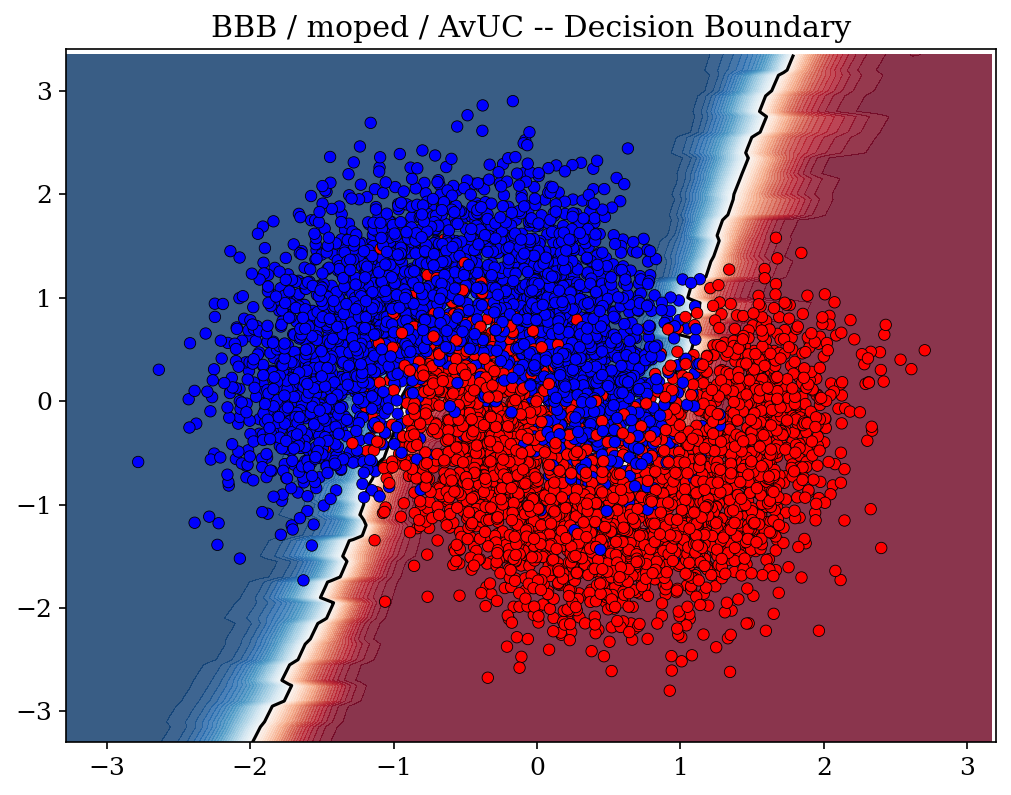
\includegraphics[width=\linewidth]{bbb_moped_avuc_boundary.png}
    \caption{BBB/MOPED/AvUC: boundary}
  \end{subfigure}\hfill
  \begin{subfigure}{0.48\linewidth}
    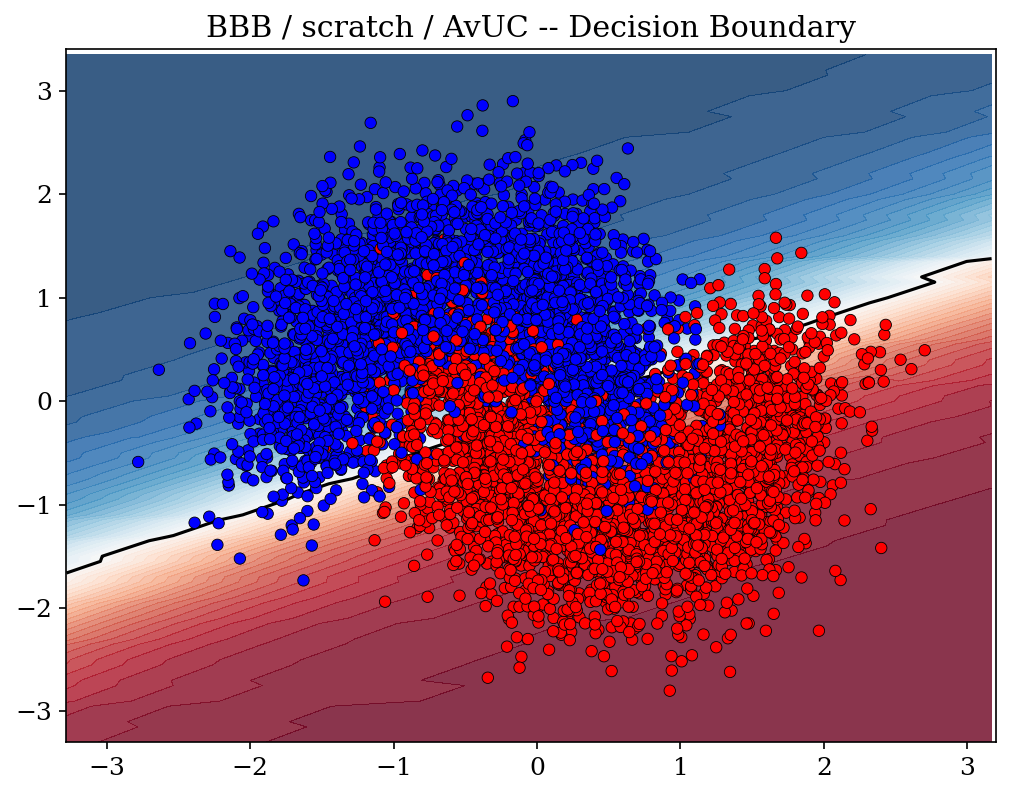
\includegraphics[width=\linewidth]{bbb_scratch_avuc_boundary.png}
    \caption{BBB/scratch/AvUC: boundary (failure)}
  \end{subfigure}
  \\[6pt]
  \begin{subfigure}{0.48\linewidth}
    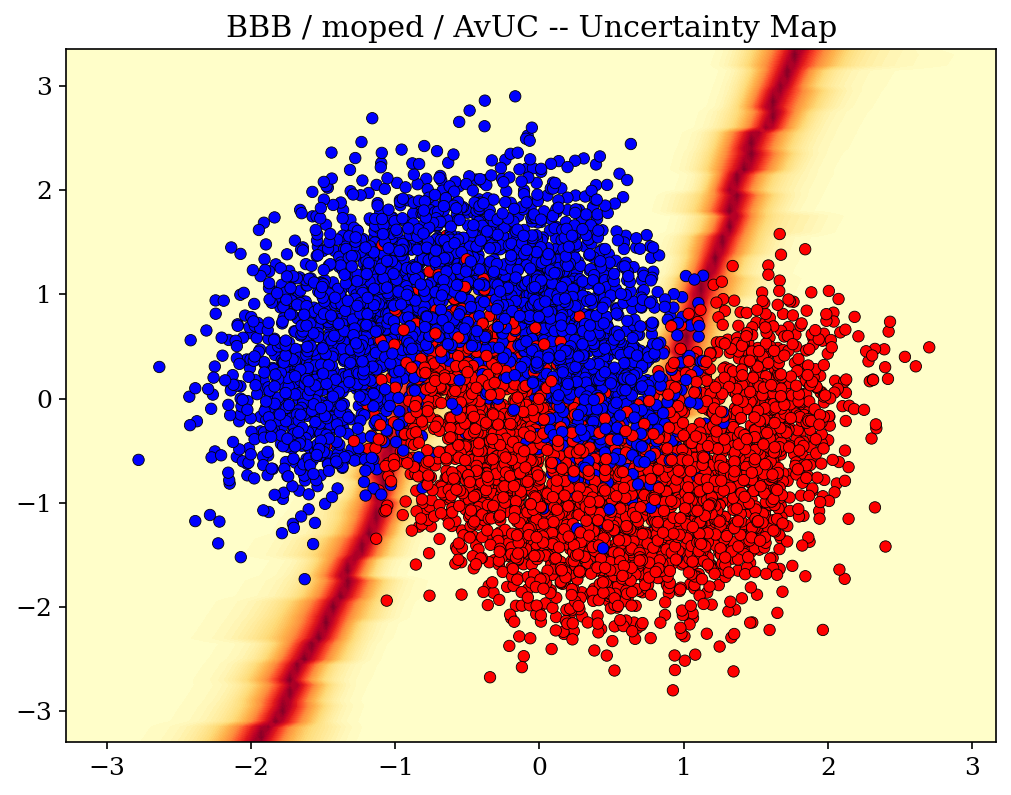
\includegraphics[width=\linewidth]{bbb_moped_avuc_uncertainty.png}
    \caption{BBB/MOPED/AvUC: uncertainty map}
  \end{subfigure}\hfill
  \begin{subfigure}{0.48\linewidth}
    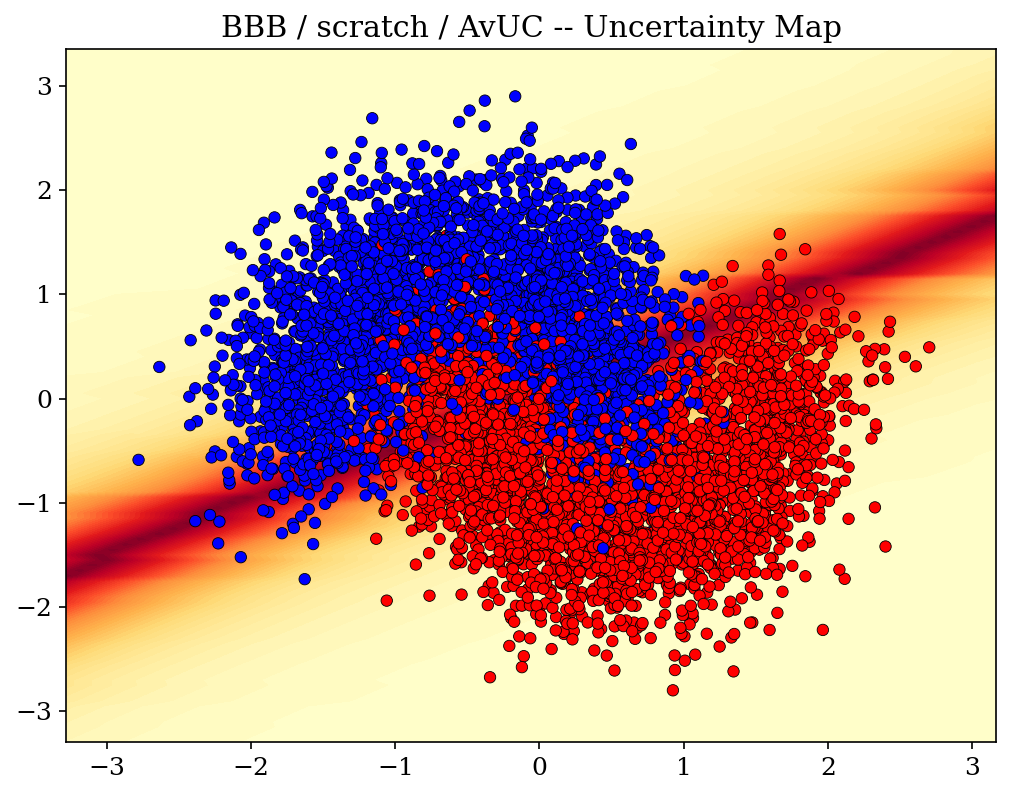
\includegraphics[width=\linewidth]{bbb_scratch_avuc_uncertainty.png}
    \caption{BBB/scratch/AvUC: uncertainty (failure)}
  \end{subfigure}
  \caption{MOPED vs.\ scratch initialisation with AvUC loss.
    Without warm-starting, AvUC collapses the posterior onto a linear
    boundary (b,d); with MOPED the non-linear crescent structure is
    recovered (a,c).}
  \label{fig:bnn_boundaries}
\end{figure}

Figure~\ref{fig:bnn_histrel} shows that BBB/MOPED/AvUC produces the sharpest
confidence histogram (almost all mass above 0.92, Conf$=0.933$) while maintaining
a roughly calibrated reliability diagram. BBB/MOPED/ELBO achieves the
cleanest reliability curve, tracking the diagonal most faithfully.

\begin{figure}[H]
  \centering
  \begin{subfigure}{0.48\linewidth}
    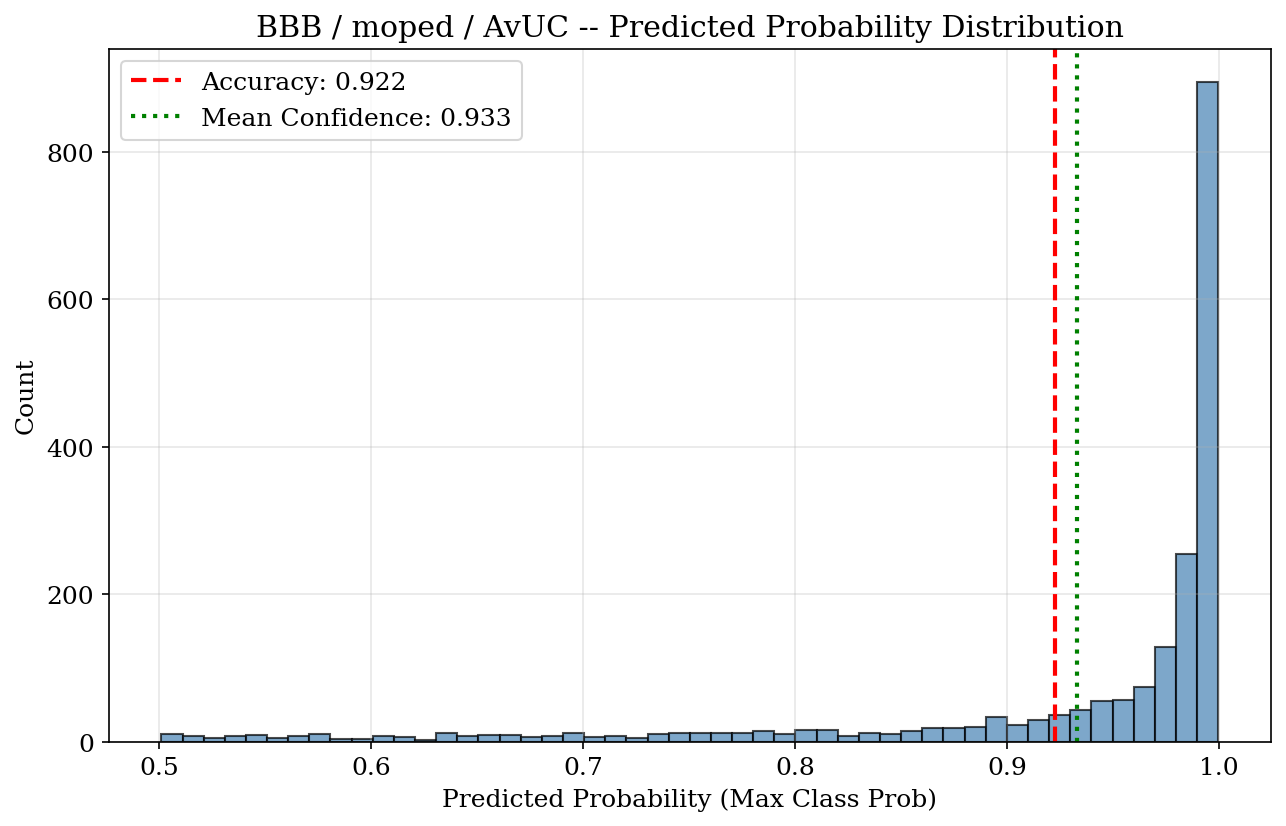
\includegraphics[width=\linewidth]{bbb_moped_avuc_histogram.png}
    \caption{BBB/MOPED/AvUC: histogram}
  \end{subfigure}\hfill
  \begin{subfigure}{0.48\linewidth}
    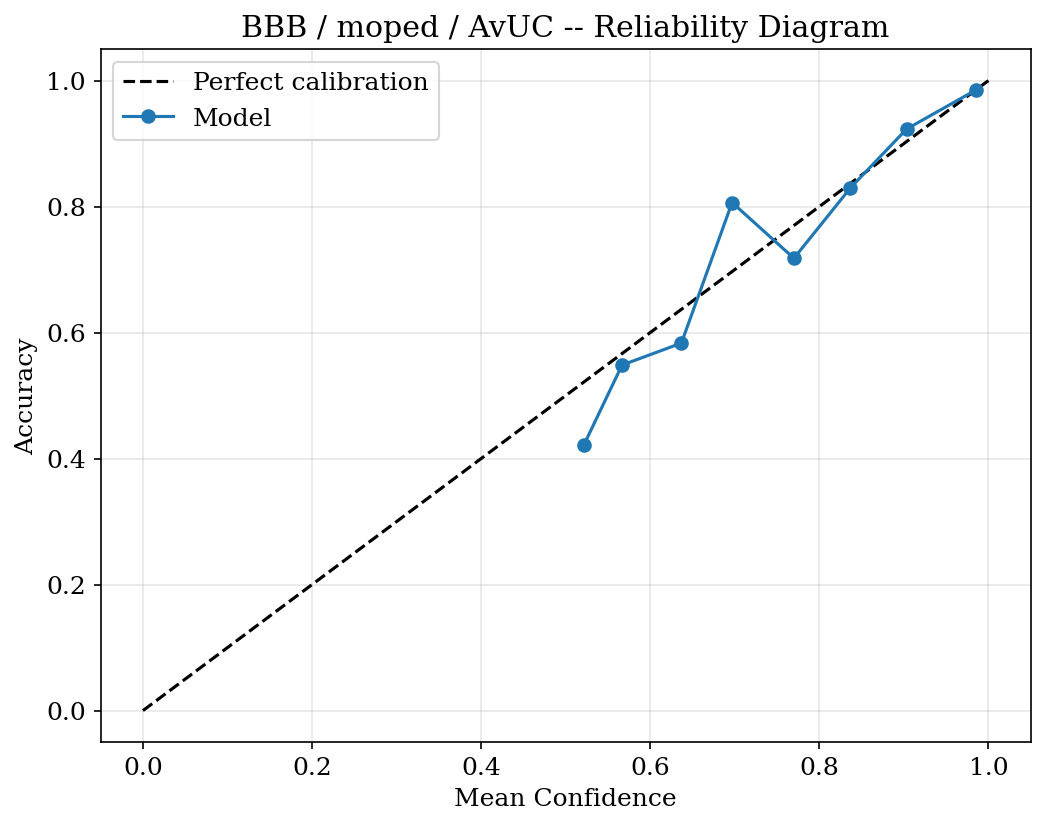
\includegraphics[width=\linewidth]{bbb_moped_avuc_reliability.png}
    \caption{BBB/MOPED/AvUC: reliability}
  \end{subfigure}
  \\[6pt]
  \begin{subfigure}{0.48\linewidth}
    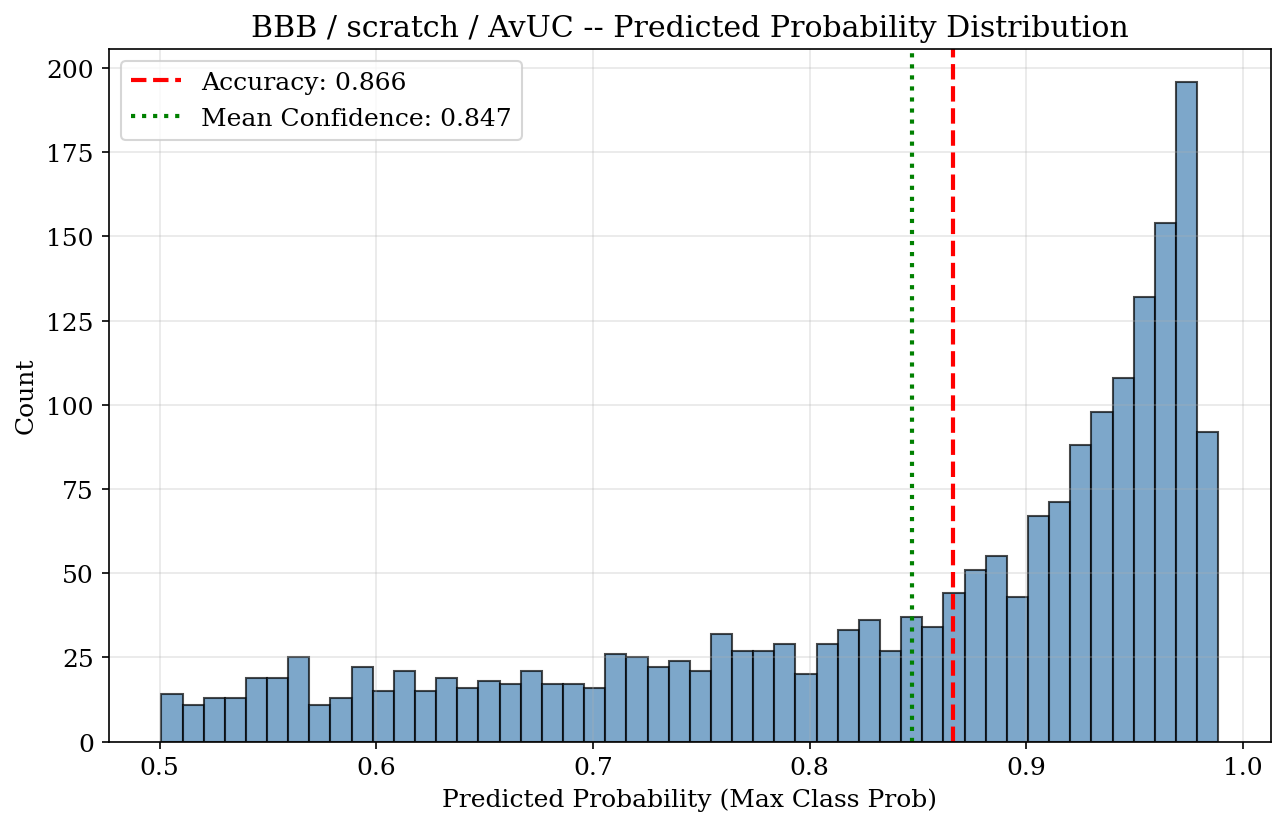
\includegraphics[width=\linewidth]{bbb_scratch_avuc_histogram.png}
    \caption{BBB/scratch/AvUC: histogram (failure)}
  \end{subfigure}\hfill
  \begin{subfigure}{0.48\linewidth}
    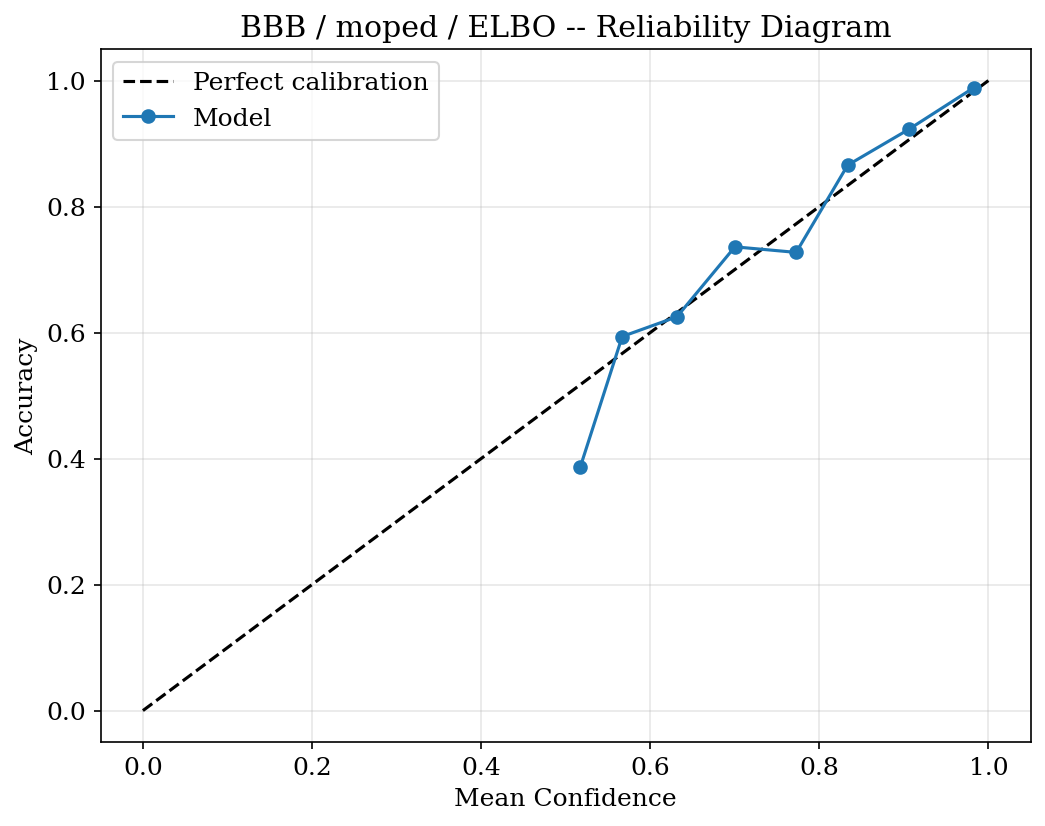
\includegraphics[width=\linewidth]{bbb_moped_elbo_reliability.png}
    \caption{BBB/MOPED/ELBO: reliability (cleanest)}
  \end{subfigure}
  \caption{Probability histograms and reliability diagrams.
    (a) BBB/MOPED/AvUC is the sharpest model; (b) its reliability is
    roughly diagonal but noisy; (c) the failure case has a broad,
    flat histogram; (d) BBB/MOPED/ELBO traces the diagonal most
    faithfully.}
  \label{fig:bnn_histrel}
\end{figure}

Figure~\ref{fig:bnn_ood} shows the epistemic uncertainty on OOD inputs
(equation~\ref{eq:mi}). All BBB variants concentrate epistemic uncertainty
at the decision boundary rather than at the OOD corners, confirming the
mean-field posterior collapse noted in Table~\ref{tab:ood}.
BBB/MOPED/AvUC reaches the highest peak mutual information ($\approx0.27$),
while BBB/scratch/ELBO shows only a thin stripe at $\leq0.068$.

\begin{figure}[H]
  \centering
  \begin{subfigure}{0.48\linewidth}
    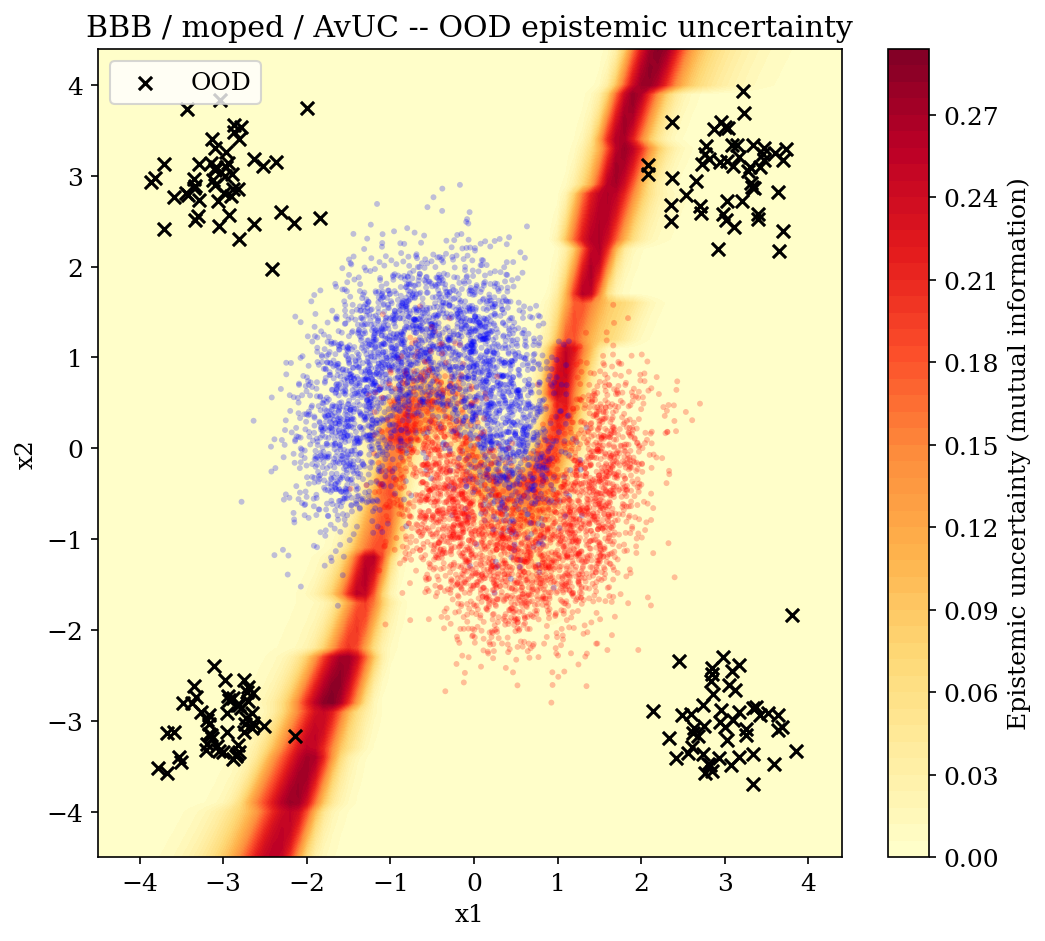
\includegraphics[width=\linewidth]{bbb_moped_avuc_ood_epistemic.png}
    \caption{BBB/MOPED/AvUC (max $\approx0.27$)}
  \end{subfigure}\hfill
  \begin{subfigure}{0.48\linewidth}
    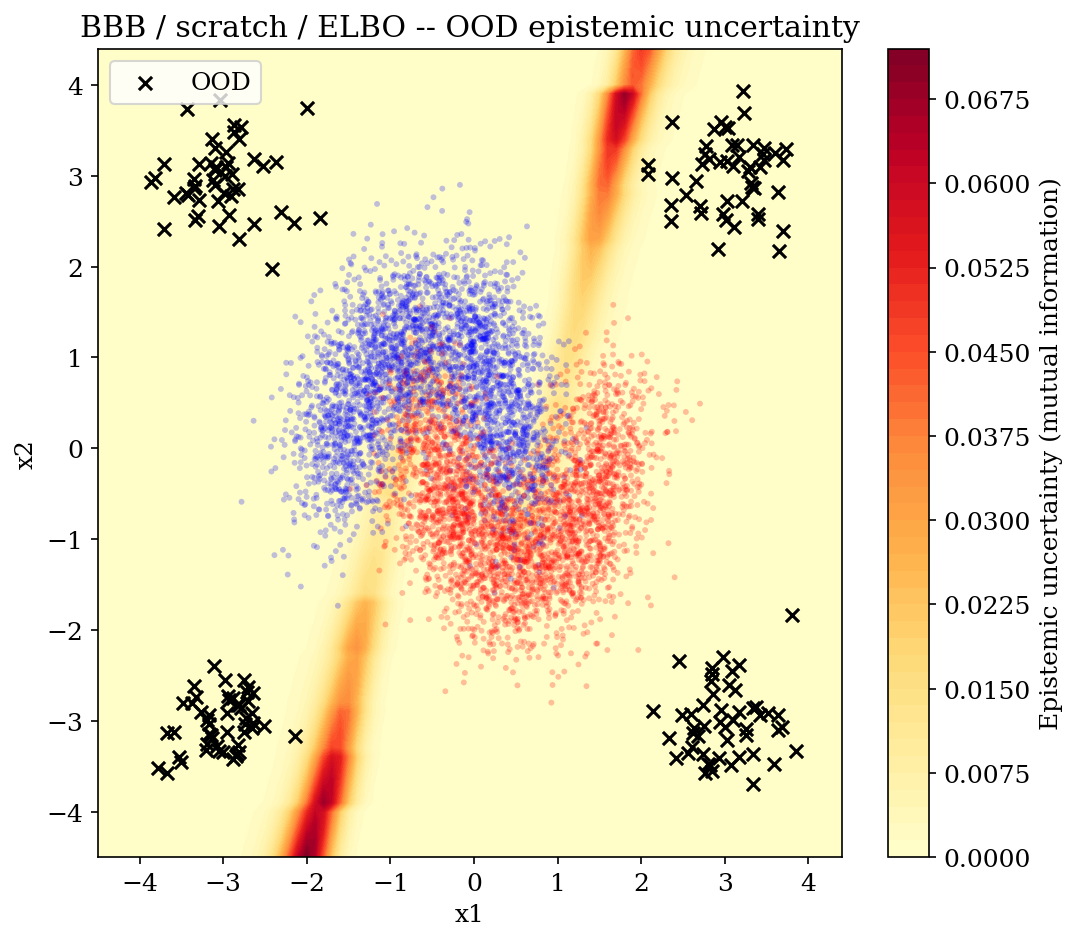
\includegraphics[width=\linewidth]{bbb_scratch_elbo_ood_epistemic.png}
    \caption{BBB/scratch/ELBO (max $\approx0.068$)}
  \end{subfigure}
  \caption{OOD epistemic uncertainty (mutual information) for two BBB
    variants. High values along the decision boundary indicate
    uncertainty about the class boundary; all OOD corner clusters
    (crosses) remain near zero, confirming posterior collapse outside
    the training region.}
  \label{fig:bnn_ood}
\end{figure}

\paragraph{Observations.}
\begin{itemize}[leftmargin=*,topsep=2pt,itemsep=1pt]
  \item \textbf{BBB/scratch/AvUC diverges} (Acc$=0.866$, flat boundary):
    AvUC's calibration objective destabilises learning without a geometric
    anchor, driving the posterior to a low-entropy linear solution that
    minimises the AU and IC counts by being uniformly uncertain everywhere.
  \item \textbf{MOPED is necessary for AvUC}: the combination
    BBB/MOPED/AvUC achieves the best NLL ($0.192$), Brier Score ($0.057$),
    and sharpest confidence ($0.933$), while ECE ($0.014$) is competitive.
  \item \textbf{BBB/MOPED/ELBO has the cleanest reliability curve}:
    its reliability diagram tracks the diagonal most faithfully, suggesting
    ELBO alone with a warm start is sufficient for good calibration at
    lower cost (15.9\,s vs.\ 68.7\,s for AvUC).
  \item \textbf{Inference cost is uniform} ($0.050$--$0.055$\,s) across
    all variants since $S=50$ MC passes are always performed.
\end{itemize}

%% ── 4.3 laplace-torch ─────────────────────────────────────────────────────
\subsection{\texttt{laplace-torch}: Laplace Approximation}
\label{sec:la}

\paragraph{Setup.}
Post-hoc fit to the shared MAP checkpoint. Ten variants cross
Hessian$\in$\{Diag, KFAC, Full\} $\times$ Scope$\in$\{all, last-layer\}
$\times$ Tuning$\in$\{grid search, marglik\}.
Prediction via \texttt{pred\_type="glm"} with probit link approximation.

\begin{lstlisting}[caption={Laplace post-hoc workflow.}]
la = Laplace(model, 'classification',
             subset_of_weights='last_layer', hessian_structure='kron')
la.fit(train_loader)
la.optimize_prior_precision(method='gridsearch', val_loader=val_loader,
                             pred_type='glm', link_approx='probit')
probs = la(X_test, pred_type='glm', link_approx='probit')
\end{lstlisting}

\paragraph{Results.}

Table~\ref{tab:la_main} reports all calibration metrics for all ten variants.
All variants share Acc$=0.92$ and MActErr$=0.08$ (not shown). U-MSE scaled
by $10^3$. Bold marks the best value per column.

\begin{sidewaystable}
  \centering
  \caption{All calibration metrics for \texttt{laplace-torch} variants on
    Two Moons. All variants achieve Acc$=0.92$ and MActErr$=0.08$.
    GS = grid search; ML = marginal likelihood; LL = last-layer.
    Bold = best per column.}
  \label{tab:la_main}
  \scriptsize\setlength{\tabcolsep}{2.5pt}
  \begin{tabular}{
    L{1.9cm} C{0.6cm} C{0.55cm}
    C{0.7cm} C{0.7cm} C{0.7cm} C{0.7cm}
    C{0.7cm} C{0.7cm} C{0.65cm}
    C{0.7cm} C{0.95cm} C{0.7cm}
    C{0.75cm} C{0.7cm}
    C{0.95cm} C{0.75cm} C{0.95cm}
  }
    \toprule
    \textbf{Variant} & \textbf{Hess} & \textbf{Sc}
      & \textbf{PP} & \textbf{NLL} & \textbf{BS} & \textbf{ECE}
      & \textbf{Conf} & \textbf{Ent} & \textbf{$1{-}c$}
      & \textbf{U-MAE} & \textbf{U-MSE}${\times}10^3$ & \textbf{U-Corr}
      & \textbf{MaxGap} & \textbf{ClECE}
      & \textbf{Fit\,(s)} & \textbf{Tune\,(s)} & \textbf{Inf\,(s)} \\
    \midrule
    \multicolumn{18}{l}{\textit{Grid search tuning ($\tau = 10^4$ for all)}} \\
    Diag/all/GS & diag & all & $10^4$ & \textbf{0.190} & \textbf{0.056} & \textbf{0.010} & 0.921 & 0.194 & 0.079 & \textbf{0.010} & 0.806 & 0.959 & 0.197 & \textbf{0.010} & 0.23  & 4.01 & 0.021 \\
    Full/all/GS & full & all & $10^4$ & \textbf{0.190} & \textbf{0.056} & \textbf{0.010} & 0.921 & 0.194 & 0.079 & \textbf{0.010} & 0.806 & 0.959 & 0.197 & \textbf{0.010} & 1263  & 11.4 & 0.034 \\
    Kron/all/GS & kron & all & $10^4$ & \textbf{0.190} & \textbf{0.056} & \textbf{0.010} & 0.921 & 0.194 & 0.079 & \textbf{0.010} & 0.806 & 0.959 & 0.197 & \textbf{0.010} & 0.54  & 5.29 & 0.022 \\
    Full/LL/GS  & full & LL  & $10^4$ & \textbf{0.190} & \textbf{0.056} & \textbf{0.010} & 0.921 & 0.194 & 0.079 & \textbf{0.010} & 0.806 & 0.959 & 0.197 & \textbf{0.010} & 7.12  & 1.52 & \textbf{0.001} \\
    \textbf{Kron/LL/GS}  & kron & LL  & $10^4$ & \textbf{0.190} & \textbf{0.056} & \textbf{0.010} & 0.921 & 0.194 & 0.079 & \textbf{0.010} & 0.806 & 0.959 & 0.197 & \textbf{0.010} & \textbf{0.43}  & 1.85 & \textbf{0.001} \\
    \multicolumn{18}{l}{\textit{Marginal likelihood tuning}} \\
    Diag/all/ML & diag & all & 8.73  & 0.192 & 0.057 & 0.016 & 0.912 & 0.219 & 0.088 & 0.016 & 0.817 & 0.955 & 0.196 & 0.016 & 0.20  & \textbf{0.06} & 0.021 \\
    Full/all/ML & full & all & 0.52  & 0.307 & 0.082 & 0.152 & 0.771 & 0.500 & 0.229 & 0.152 & 26.0  & 0.913 & 0.218 & 0.152 & 1122  & 1.88 & 0.034 \\
    Kron/all/ML & kron & all & 1.42  & 0.238 & 0.065 & 0.086 & 0.841 & 0.377 & 0.159 & 0.086 & 9.07  & 0.923 & 0.152 & 0.086 & 0.53  & 0.10 & 0.022 \\
    Full/LL/ML  & full & LL  & 1.79  & 0.226 & 0.062 & 0.070 & 0.855 & 0.348 & 0.145 & 0.070 & 6.49  & 0.935 & 0.136 & 0.070 & 7.13  & 0.09 & \textbf{0.001} \\
    Kron/LL/ML  & kron & LL  & 2.04  & 0.221 & 0.061 & 0.064 & 0.862 & \textbf{0.334} & 0.138 & 0.064 & 5.50  & 0.938 & \textbf{0.141} & 0.064 & 0.44  & \textbf{0.08} & \textbf{0.001} \\
    \bottomrule
  \end{tabular}
  \begin{flushleft}\footnotesize
    Sc = weight scope; LL = last-layer; PP = tuned prior precision.
    U-MSE scaled by $10^3$. MaxGap = max binned uncertainty gap.
    ClECE = classwise ECE. All GS variants converge to $\tau=10^4$;
    metric differences among them are due to floating-point noise only.
  \end{flushleft}
\end{sidewaystable}

\paragraph{The marginal likelihood failure case.}
Figure~\ref{fig:la_failure} visualises the Full/all/marglik failure
(ECE$=0.152$, $\tau=0.52$). The marginal likelihood selects a prior
precision nearly $10{,}000\times$ smaller than grid search ($\tau=10^4$),
inflating the posterior so severely that the decision boundary shifts far
off the data and the reliability curve swings far above the diagonal
(underconfident).

\begin{figure}[H]
  \centering
  \begin{subfigure}{0.48\linewidth}
    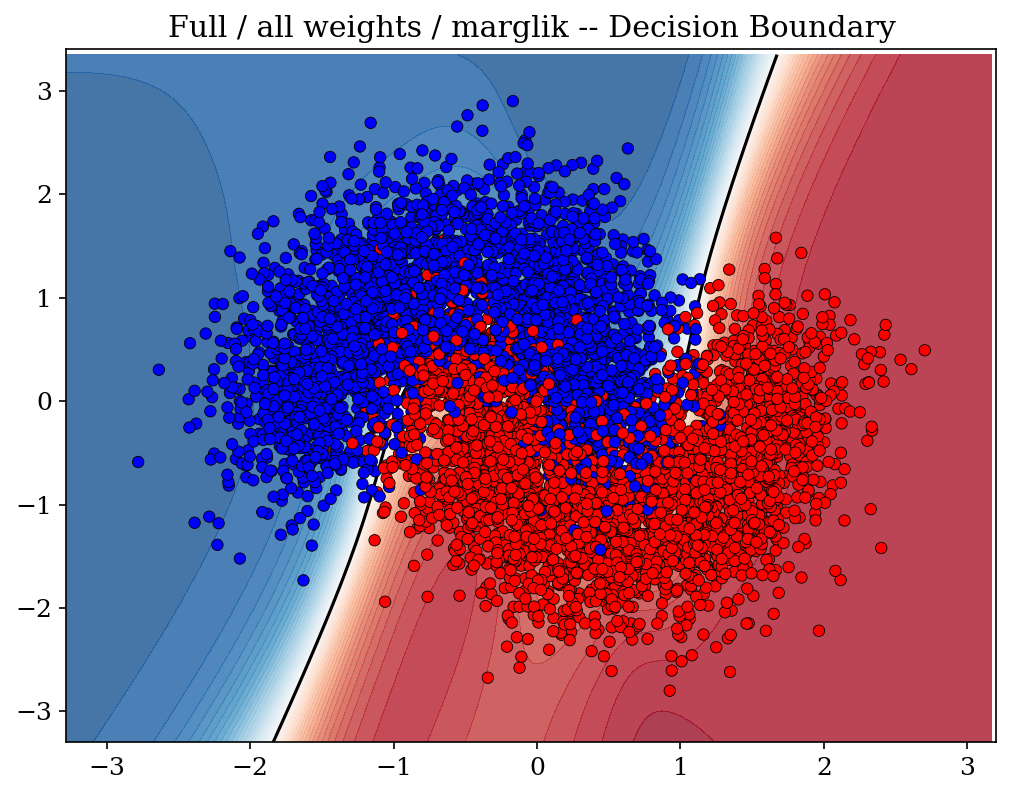
\includegraphics[width=\linewidth]{marglik_full_all_weights_boundary.png}
    \caption{Full/all/marglik: decision boundary}
  \end{subfigure}\hfill
  \begin{subfigure}{0.48\linewidth}
    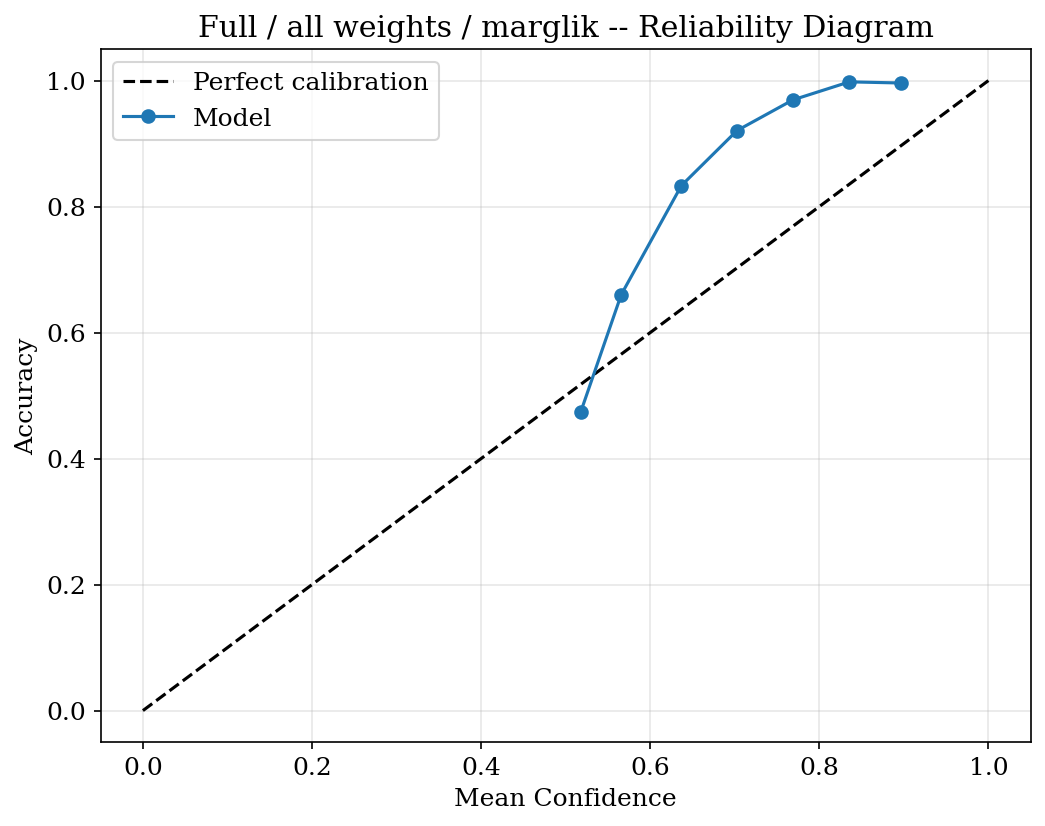
\includegraphics[width=\linewidth]{marglik_full_all_weights_reliability.png}
    \caption{Full/all/marglik: reliability diagram}
  \end{subfigure}
  \caption{Marginal likelihood failure for Full/all LA ($\tau=0.52$).
    The over-diffuse posterior shifts the boundary to the right (a) and
    produces a strongly underconfident reliability curve (b);
    compare the target diagonal.}
  \label{fig:la_failure}
\end{figure}

\paragraph{Characteristic uncertainty pattern.}
All marglik-tuned variants share a visually striking feature: the uncertainty
map collapses to a razor-thin stripe along the decision boundary, with the
rest of the input space (including OOD regions) essentially at zero
(Figure~\ref{fig:la_stripe}). This is the spatial signature of the small
$\tau$ values selected by marglik, which keep the posterior very close to
the MAP.

\begin{figure}[H]
  \centering
  \begin{subfigure}{0.48\linewidth}
    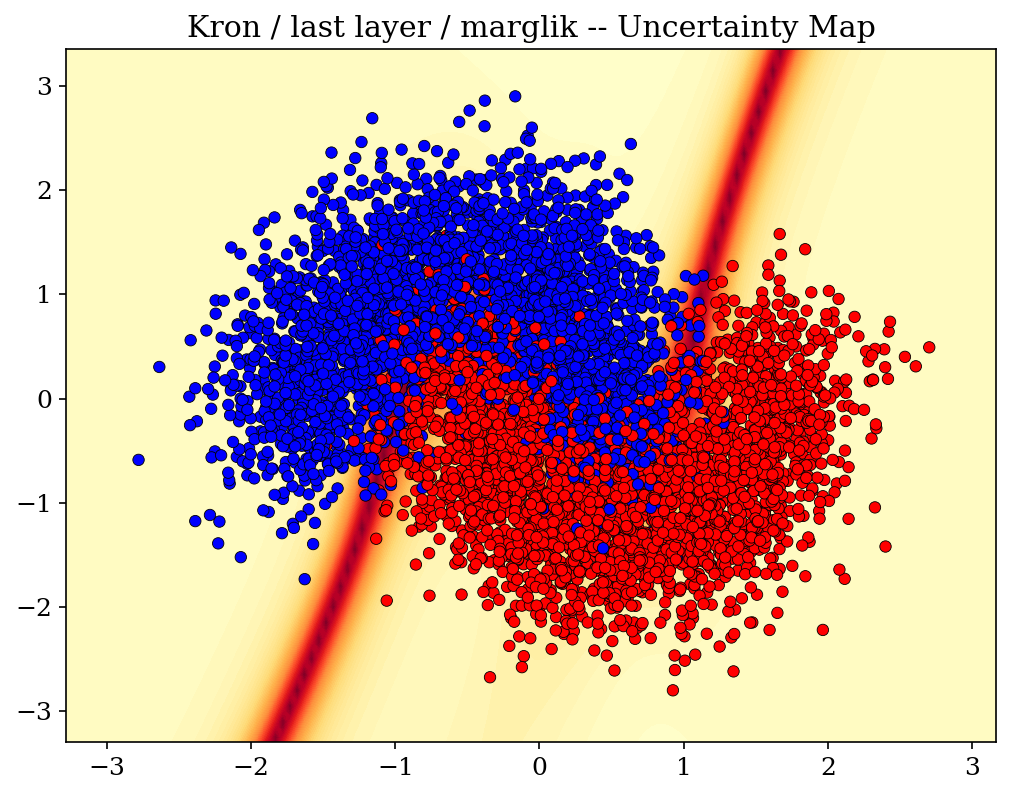
\includegraphics[width=\linewidth]{marglik_kron_last_layer_uncertainty.png}
    \caption{Kron/LL/marglik}
  \end{subfigure}\hfill
  \begin{subfigure}{0.48\linewidth}
    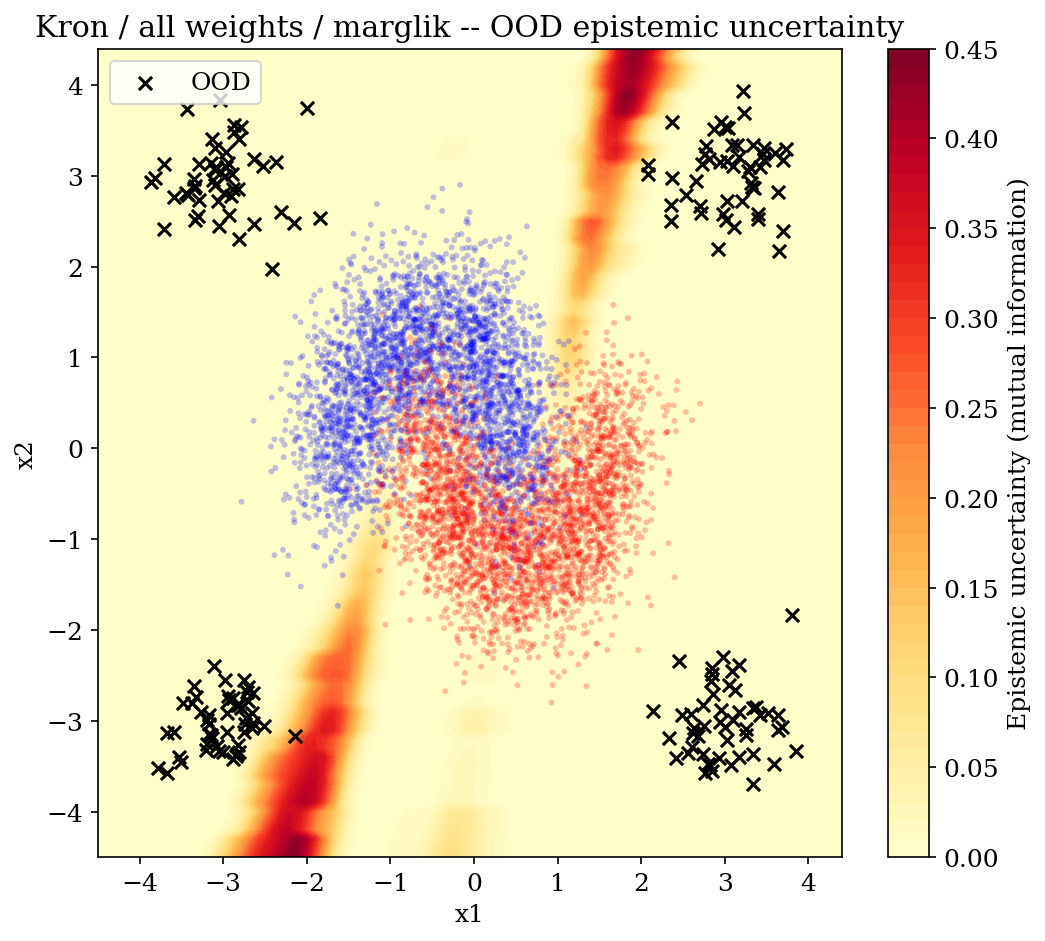
\includegraphics[width=\linewidth]{marglik_kron_all_weights_ood_epistemic.png}
    \caption{Kron/all/marglik OOD epistemic (max $\approx0.45$)}
  \end{subfigure}
  \caption{Uncertainty patterns under marginal likelihood tuning.
    (a)~All marglik variants show a narrow stripe; outside it the model
    is maximally confident. (b)~Surprisingly, Kron/all marglik does
    detect OOD in the corners (mutual information up to $0.45$):
    the all-weights posterior retains some OOD sensitivity despite
    marglik's tendency towards diffuse priors.}
  \label{fig:la_stripe}
\end{figure}

\paragraph{Observations.}
\begin{itemize}[leftmargin=*,topsep=2pt,itemsep=1pt]
  \item \textbf{All grid-search variants are identical} (ECE$=0.010$,
    NLL$=0.190$): all converge to $\tau=10^4$. Hessian structure and scope
    affect only fit cost, not calibration quality.
  \item \textbf{Full/all/marglik catastrophically fails}: $\tau=0.52$,
    Conf$=0.771$, Ent$=0.500$ (maximum binary entropy). The full GGN
    evidence landscape is poorly conditioned for this network.
  \item \textbf{KFAC marglik is more robust} ($\tau\in[1.4,2.0]$,
    ECE$\leq0.086$); the Kronecker structure regularises the landscape.
  \item \textbf{Kron/LL/GS is Pareto-optimal}: best calibration at lowest
    cost (fit $0.43$\,s, tune $1.85$\,s, inference $<1$\,ms).
  \item \textbf{OOD split by scope}: all-weights marglik variants preserve
    OOD epistemic sensitivity; last-layer variants collapse to near-zero
    outside the boundary stripe.
\end{itemize}

\subsection{Cross-Library Summary}

\begin{table}[H]
  \centering
  \caption{Best representatives vs.\ MAP baseline on Two Moons.}
  \label{tab:cross}
  \small\setlength{\tabcolsep}{4pt}
  \begin{tabular}{L{3.8cm} C{0.8cm} C{0.8cm} C{0.8cm} C{0.8cm}
                  C{0.8cm} C{0.8cm} C{1.4cm} C{1.4cm}}
    \toprule
    \textbf{Model} & \textbf{Acc} & \textbf{NLL} & \textbf{BS}
      & \textbf{ECE} & \textbf{Conf} & \textbf{Ent}
      & \textbf{Fit\,(s)} & \textbf{Inf\,(s)} \\
    \midrule
    MAP baseline           & 0.92 & $\sim$0.20 & $-$ & $-$ & $-$ & $-$ & 33.6 & $<$0.001 \\
    \midrule
    BBB / MOPED / AvUC  & \textbf{0.923} & 0.192 & \textbf{0.057} & 0.014
      & \textbf{0.933} & \textbf{0.173} & 68.7 & 0.051 \\
    \midrule
    Kron / LL / GS      & 0.920 & \textbf{0.190} & \textbf{0.056} & \textbf{0.010}
      & 0.921 & 0.194 & \textbf{0.43} & \textbf{0.001} \\
    \bottomrule
  \end{tabular}
\end{table}

The LA (Kron/LL/GS) matches or exceeds best SVI calibration at
$\mathbf{\approx200\times}$ lower fit cost and $\mathbf{\approx60\times}$
lower inference cost. BBB/MOPED/AvUC achieves marginally higher confidence
and lower entropy, indicating a sharper posterior, at the cost of full
retraining with multiple MC forward passes per step.

%% ───────────────────────────────────────────────────────────────────────────
\section{Toy Regression Experiment}
\label{sec:regression}

\todo{To be written. 1-D/2-D regression notebooks: dataset, predictive
  mean/variance plots, NLL and RMSE tables for both libraries.}

%% ───────────────────────────────────────────────────────────────────────────
\section{PovertyMap Replication (Laplace Redux)}
\label{sec:povertymap}

\todo{To be written. Replicates distribution-shift experiments
  from~\citet{daxberger2021laplace} on PovertyMap: ResNet backbone,
  in-distribution and OOD metrics, comparison against paper numbers.}

%% ───────────────────────────────────────────────────────────────────────────
\section{Discussion}
\label{sec:discussion}

\todo{Full discussion pending regression and PovertyMap results.}

\paragraph{Post-hoc vs.\ by-design.}
\texttt{laplace-torch} imposes near-zero training overhead~\citep{daxberger2021laplace}.
\texttt{bayesian-torch} requires modified training, doubles parameters, but
provides a full variational posterior and the AvUC calibration
objective~\citep{intel2021bayesiantorch,blundell2015weight}.

\paragraph{MOPED as a geometric anchor.}
The BBB/scratch/AvUC failure demonstrates that AvUC's calibration term alone
is not sufficient: without MOPED's warm start, the AvUC objective can be
minimised by collapsing to an incorrect but low-entropy linear boundary.
MOPED should be considered mandatory when training with AvUC.

\paragraph{Hessian structure and marglik conditioning.}
Under grid search, structure does not matter for Two Moons.
Under marglik, full-matrix GGN curvature is poorly conditioned and selects
pathological prior precisions; KFAC regularises the evidence landscape.

\paragraph{OOD uncertainty: a key divergence.}
All-weights LA marglik variants retain some OOD epistemic sensitivity
(mutual information up to $0.45$ in corners), while last-layer LA
and all SVI variants collapse to near-zero outside the boundary.
This is a critical distinction for safety-critical applications.

%% ───────────────────────────────────────────────────────────────────────────
\section{Conclusion}
\label{sec:conclusion}

\todo{To be written once regression and PovertyMap sections are complete.}

%% ───────────────────────────────────────────────────────────────────────────
\appendix


\bibliographystyle{plainnat}
\bibliography{references}

\end{document}